% ------------------------------------------------------------------------------
% TYPO3 CMS 7.5 - What's New - Chapter "Introduction" (Serbian Version)
%
% @author	Michael Schams <schams.net>
% @license	Creative Commons BY-NC-SA 3.0
% @link		http://typo3.org/download/release-notes/whats-new/
% @language	Serbian
% ------------------------------------------------------------------------------
% LTXE-CHAPTER-UID:		3a84d600-9fb67dda-31c4af65-dd7a4af5
% LTXE-CHAPTER-NAME:	Introduction
% ------------------------------------------------------------------------------

\section{Uvod}
\begin{frame}[fragile]
	\frametitle{Uvod}

	\begin{center}\huge{Uvod}\end{center}
	\begin{center}\huge{\color{typo3darkgrey}\textbf{Cinjenice}}\end{center}

\end{frame}

% ------------------------------------------------------------------------------
% LTXE-SLIDE-START
% LTXE-SLIDE-UID:		1f19681c-061b29b4-3e0f52bb-dcee978f
% LTXE-SLIDE-ORIGIN:	81d53787-fb3806f0-841b4042-7033fad4 English
% LTXE-SLIDE-ORIGIN:	f1ea1041-2b6b2b81-f54b45c0-84265d6a German
% LTXE-SLIDE-TITLE:		TYPO3 CMS 7.5 - The Facts
% ------------------------------------------------------------------------------
\begin{frame}[fragile]
	\frametitle{Uvod}
	\framesubtitle{TYPO3 CMS 7.5 - Cinjenice}

	\begin{itemize}
		\item Datum objavljivanja: 29. September 2015
		\item Tip objavljivanja: "Brza objava" ("Sprint Release")
		\item Vizija: Prihvatiti, inovirati, dostaviti
		\item Glavni fokus: Finalizacija
	\end{itemize}

	\begin{figure}
		
\includegraphics[width=0.95\linewidth]{Introduction/typo3cms75-banner.jpg}
	\end{figure}

\end{frame}

% ------------------------------------------------------------------------------
% LTXE-SLIDE-START
% LTXE-SLIDE-UID:		3568eea8-14389548-a4a6d858-1085160a
% LTXE-SLIDE-ORIGIN:	a0327db8-b4a9bd42-f32515d0-87296684 English
% LTXE-SLIDE-ORIGIN:	5d8adc7d-af29cb46-4acd2255-27362935 German
% LTXE-SLIDE-TITLE:		System Requirements
% ------------------------------------------------------------------------------
\begin{frame}[fragile]
	\frametitle{Uvod}
	\framesubtitle{Sistemski zahtevi}

	\begin{itemize}
		\item PHP*:\tabto{3cm}v5.5.0 - v5.6.x
		\item MySQL:\tabto{3cm}v5.5.x - v5.6.x (no strict mode)
		\item Prostor na disku:\tabto{3cm}min 200 MB
		\item PHP podesavanja:

			\begin{itemize}
				\item memory\_limit >= 128M
				\item max\_execution\_time >= 240s
				\item opcija \texttt{--disable-ipv6} \underline{ne sme} se koristit
			\end{itemize}

		\item Administratorski interfejs zahteva IE >= 9 ili bilo koji drugi moderni pretrazivac

	\end{itemize}

	\vspace{1cm}

	*) Dodatno objasnjenje: \href{http://typo3.org/news/article/php-minimum-requirements-for-typo3-cms-7/}{PHP Minimum Requirements for TYPO3 CMS 7}

\end{frame}

% ------------------------------------------------------------------------------
% LTXE-SLIDE-START
% LTXE-SLIDE-UID:		a18f63ec-53d50ad1-b9ab1386-a0d7d41f
% LTXE-SLIDE-ORIGIN:	c155d534-1a53682d-f56423dc-163111d3 English
% LTXE-SLIDE-ORIGIN:	6cad14bf-08874e74-1dd85333-e5c43a08 German
% LTXE-SLIDE-TITLE:		Development And Release Timeline
% ------------------------------------------------------------------------------
\begin{frame}[fragile]
	\frametitle{Uvod}
	\framesubtitle{Vreme razvoja i datumi objavljivanja}

	\begin{figure}
		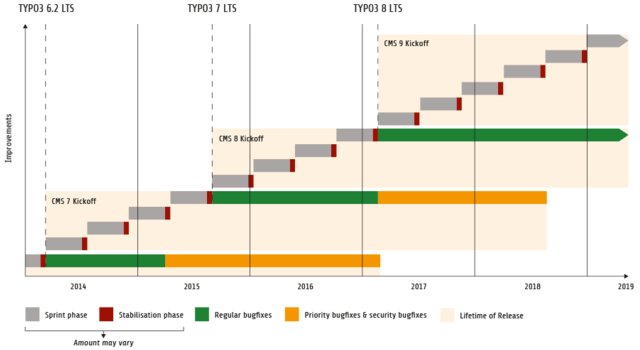
\includegraphics[width=0.90\linewidth]{Introduction/ReleaseAgenda.png}
	\end{figure}

\end{frame}

% ------------------------------------------------------------------------------
% LTXE-SLIDE-START
% LTXE-SLIDE-UID:		b85f7770-647d875f-69714254-44359327
% LTXE-SLIDE-ORIGIN:	83c1fb1c-ed592fa9-a2a279bd-be5cc800 English
% LTXE-SLIDE-ORIGIN:	387f7aeb-53ab533f-95427547-3aa76412 German
% LTXE-SLIDE-TITLE:		TYPO3 CMS Roadmap
% ------------------------------------------------------------------------------
\begin{frame}[fragile]
	\frametitle{Uvod}
	\framesubtitle{TYPO3 CMS plan}

	Predvidjeni datumi objavljivanja i njihov osnovni fokus:

	\begin{itemize}
		\item v7.0 \tabto{1.1cm}02/Dec/2014\tabto{3.4cm}Remont administratorskog interfejsa prvi deo
		\item v7.1 \tabto{1.1cm}24/Feb/2015\tabto{3.4cm}Ciscenje osnove sistema i optimizacija
		\item v7.2 \tabto{1.1cm}28/Apr/2015\tabto{3.4cm}Korisnicki interfejs
		\item v7.3 \tabto{1.1cm}16/Jun/2015\tabto{3.4cm} Ekosistem za dodatke, Composer\newline
			\tabto{3.4cm} i upravljanje prosirenjima
		\item v7.4 \tabto{1.1cm}04/Aug/2015\tabto{3.4cm}Remont administratorskog interfejsa drugi deo

		\item
			\begingroup
				\color{typo3orange}
					v7.5 \tabto{1.1cm}29/Sep/2015\tabto{3.4cm}Finalizacija
			\endgroup

		\item v7 LTS \tabto{1.1cm}Oct/Nov/2015\tabto{3.4cm}\textbf{TYPO3 CMS 7 LTS} (Long Term Release)
	\end{itemize}

	\smaller
		\url{https://typo3.org/typo3-cms/roadmap/}\newline
		\url{http://typo3.org/news/article/embrace-and-innovate-typo3-cms-7/}
	\normalsize

\end{frame}

% ------------------------------------------------------------------------------
% LTXE-SLIDE-START
% LTXE-SLIDE-UID:		b2ae2d64-8a6051b8-93b0e424-23df3a19
% LTXE-SLIDE-ORIGIN:	63decc15-57478e30-70c7ae99-27abd3c2 English
% LTXE-SLIDE-ORIGIN:	3b01edfd-6f06e241-2670b2ad-1b598b4e German
% LTXE-SLIDE-TITLE:		Installation
% ------------------------------------------------------------------------------
\begin{frame}[fragile]
	\frametitle{Uvod}
	\framesubtitle{Instalacija}

	\begin{itemize}
		\item Zvanicna procedura za instalaciju na Linux/Mac OS X\newline
			(DocumentRoot na primer \texttt{/var/www/site/htdocs}):
		\begin{lstlisting}
			$ cd /var/www/site
			$ wget --content-disposition get.typo3.org/7.5
			$ tar xzf typo3_src-7.5.0.tar.gz
			$ cd htdocs
			$ ln -s ../typo3_src-7.5.0 typo3_src
			$ ln -s typo3_src/index.php
			$ ln -s typo3_src/typo3
			$ touch FIRST_INSTALL
		\end{lstlisting}

		\item Simbolicki linkovi (Symbolic links) na Microsoft Windows:

			\begin{itemize}
				\item Koristiti \texttt{junction} za Windows XP/2000
				\item Koristiti \texttt{mklink} za Windows Vista i Windows 7
			\end{itemize}

	\end{itemize}
\end{frame}

% ------------------------------------------------------------------------------
% LTXE-SLIDE-START
% LTXE-SLIDE-UID:		49868b71-9465dc75-066ed95d-32e1c618
% LTXE-SLIDE-ORIGIN:	4dbfb1f2-70930473-ec804474-1c2ac93a English
% LTXE-SLIDE-ORIGIN:	22ce445c-fe028a61-d11c8f8c-510270d3 German
% LTXE-SLIDE-TITLE:		Upgrade to TYPO3 CMS 7
% ------------------------------------------------------------------------------
\begin{frame}[fragile]
	\frametitle{Uvod}
	\framesubtitle{Nadogradnja na TYPO3 CMS 7.x}

	\begin{itemize}
		\item Nadogradnja je moguca samo sa TYPO3 CMS 6.2 LTS
		\item TYPO3 CMS < 6.2 bi prvo trebalo nadograditi na TYPO3 CMS 6.2 LTS
	\end{itemize}

	\begin{itemize}

		\item Upsutstvo za nadogradnju:\newline
			\smaller\url{http://wiki.typo3.org/Upgrade#Upgrading_to_7.5}\normalsize
		\item Zvanicni TYPO3 vodic "TYPO3 Installation and Upgrading":
			\smaller\url{http://docs.typo3.org/typo3cms/InstallationGuide}\normalsize
		\item Opsti pristup:
			\begin{itemize}
				\item Proveriti minimalne sistemske zahte \small(PHP, MySQL, itd.)
				\item Proveriti \textbf{deprecation\_*.log} u staroj TYPO3 instanci
				\item Nadograditi sva prosirenja na najnoviju verziju
				\item Postaviti nove fajlove i pokrenuti Install Tool \textrightarrow Upgrade Wizard
				\item Proveriti startup modul za administratore (opciono)
			\end{itemize}
	\end{itemize}

\end{frame}

% ------------------------------------------------------------------------------
